%!TEX root = ../article/Journal_SelfCalibration.tex



\section{Results}
\label{sec:results}

\subsection{EEG results} Fig. \ref{fig:EEGresults} shows the grand-averaged signals obtained during the online experiments. Error and correct assessments generated different evoked responses posterior to the device actions. The difference between error and correct potentials appeared on fronto-central locations at around 400 and 600 ms, where the error potential exhibited significantly larger positive and negative peaks respectively (unpaired t-tests, p$<1 \cdot 10^{-6}$). These evoked responses were in line with previous experiments using error potentials \cite{chavarriaga2010learning, iturrate13}.

\begin{samepage}
\begin{figure*}[!htbp]
\centering
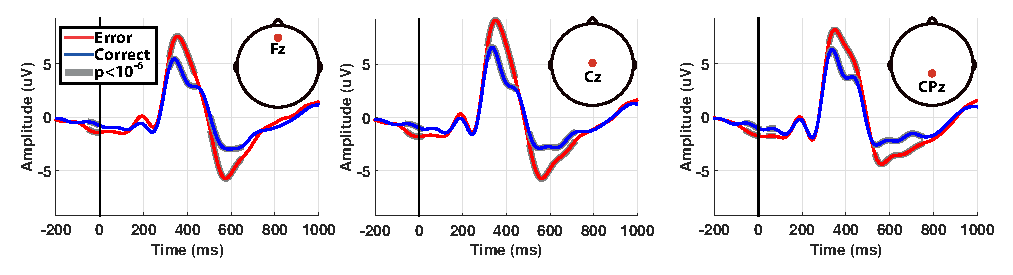
\includegraphics[width=\textwidth]{figures/EEG_results.eps}
\caption{\textbf{Grand-averaged signals for Fz, FCz and CPz channels}. Red and blue lines represent averaged signals for the error and correct conditions respectively, where the movement onset is marked as time 0 ms. Statistical differences (unpaired t-tests, p-values$<1\cdot10^{-6}$) between error and correct averages are marked by shadowed areas.}
\label{fig:EEGresults}
\end{figure*}

\begin{table*}
	\centering
	\caption{\label{tab:onlineXPsummary} Task results}
	\rowcolors{2}{gray!25}{white}
	\resizebox{\textwidth}{!}{
	\begin{tabular}{ccccc|cccc}
		\toprule
		& \multicolumn{4}{c}{\textbf{Online self-calibration}}
		& \multicolumn{4}{c}{\textbf{Simulated standard calibration}} \\ \midrule
		\textbf{Subject} & Calib. trials & Steps $1^{st}$ & $\#$Correct & $\#$Incorrect
		& Calib. trials & Steps $1^{st}$ & $\#$Correct & $\#$Incorrect \\ \midrule
		\textbf{S1} & 0 & 101 & 16 & 2 &  213 & 239.71 $\pm$ 9.2 & 10.33 $\pm$ 1.48 & 0.14 $\pm$ 0.38\\
		\textbf{S2} & 0 & 131 & 9 & 1 &  246 & 286.73 $\pm$ 14.75 & 5.50 $\pm$ 0.93 & 0.03 $\pm$ 0.22\\
		\textbf{S3} & 0 & 265 & 3 & 1 & 190 & 323.67 $\pm$ 56.32 & 1.78 $\pm$ 0.76 & 0.01 $\pm$ 0.10\\
		\textbf{S4} & 0 & 232 & 2 & 2 & 101 & 336.98 $\pm$ 75.50 & 0.59 $\pm$ 0.71 & 0.10 $\pm$ 0.33\\
		\textbf{S5} & 0 & 132 & 5 & 3 & 234 & 317.68 $\pm$ 24.85 & 2.60 $\pm$ 0.83 & 0.02 $\pm$ 0.14\\
		\textbf{S6} & 0 & 142 & 10 & 0 & 300 & 340.31 $\pm$ 15.08 & 4.62 $\pm$ 0.81 & 0.09 $\pm$ 0.29\\
		\textbf{S7} & 0 & 79 & 4 & 3 & 82 & 310.24 $\pm$ 103.64 & 0.48 $\pm$ 0.82 & 0.36 $\pm$ 0.66\\
		\textbf{S8} & 0 & 240 & 6 & 0 & 252 & 290.47 $\pm$ 12.7 & 5.91 $\pm$ 0.70 & 0.05 $\pm$ 0.22\\
		\textbf{mean} & \textbf{0.00} & \textbf{165.25} & \textbf{6.88} & \textbf{1.50}
					  & \textbf{202.25} & \textbf{305.72 $\pm$ 32.97} & \textbf{3.97 $\pm$ 3.32} & \textbf{0.10 $\pm$ 0.11} \\ \bottomrule
	\end{tabular}}
\end{table*}

\end{samepage}

\subsection{Online self-calibration results}

Table \ref{tab:onlineXPsummary}, left shows the results obtained during the online experiments. On average, users were able to reach $6.88$ correct targets in the 500 steps of the experiment. However, users also reached an average of $1.50$ incorrect targets, significantly greater than zero (one-sample t-test, $t_{7} = 3.55, p=0.009$). Whereas users needed 165 steps on average to reach the first target, subsequent targets were reached after 60 $\pm$ 24 steps on average across subjects. Note that the first target needed a substantially larger amount of data to converge due to the uncertainty not only on the target to reach, but also on the decoder of brain signals.

Fig. \ref{fig:percentage_errors} shows the evolution of the ratio of errors within the last ten movements of the device until reaching the first target. The results for each subject show a clear decreasing trend in the percentage of errors significant for all the subjects ($p<0.001$) with an average correlation of $r=0.57 \pm 0.17$. Expectedly, these results show that the error rate was variable throughout the experiment. Nonetheless, the negative tendency also indicated that the system was able to iteratively learn the task even for the first target using completely unsupervised data. Regarding the labels quality, Fig. \ref{fig:labels}a shows the ten-fold accuracy obtained with the ground truth labels, compared against the percentage of labels correctly learned by the self-calibration protocol. The results show an almost significant correlation between the two variables ($r = 0.69, p=0.06$). Nonetheless, the ratio of labels correctly assigned was always higher than $90\%$, indicating that even for subjects with low accuracies ($<60\%$), most of the labels are correctly estimated.
%
Fig. \ref{fig:labels}b shows the ten-fold accuracy obtained with ground truth labels versus the accuracy obtained with the labels estimated from self-calibration. Interestingly, there seemed to be two clusters of subjects: those who were not affected by the labeling quality composed of five subjects with very similar accuracies to the ones obtained with ground truth labels, even when not all the labels were correctly assigned; and other subjects where the labeling of the self-calibration approach affected the separability of the data acquired with a decrease of $8.41\%$ of accuracy on average.

\begin{figure*}[!ht]
		\centering
		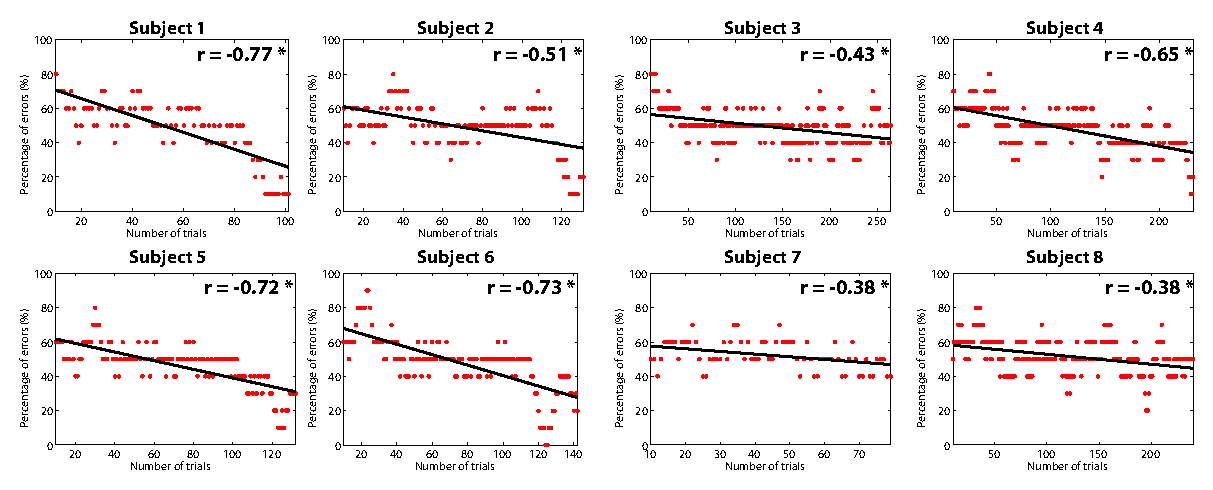
\includegraphics[width=\textwidth]{figures/percentage_errors.eps}
		\caption{\label{fig:percentage_errors} \textbf{Percentage of errors performed by the device during the last 10 trials}, as a function of the number of trials (only during the first target). Additionally, the tendency line and the correlation value are also shown.}
\end{figure*}


\begin{figure*}[!htbp]
\centering
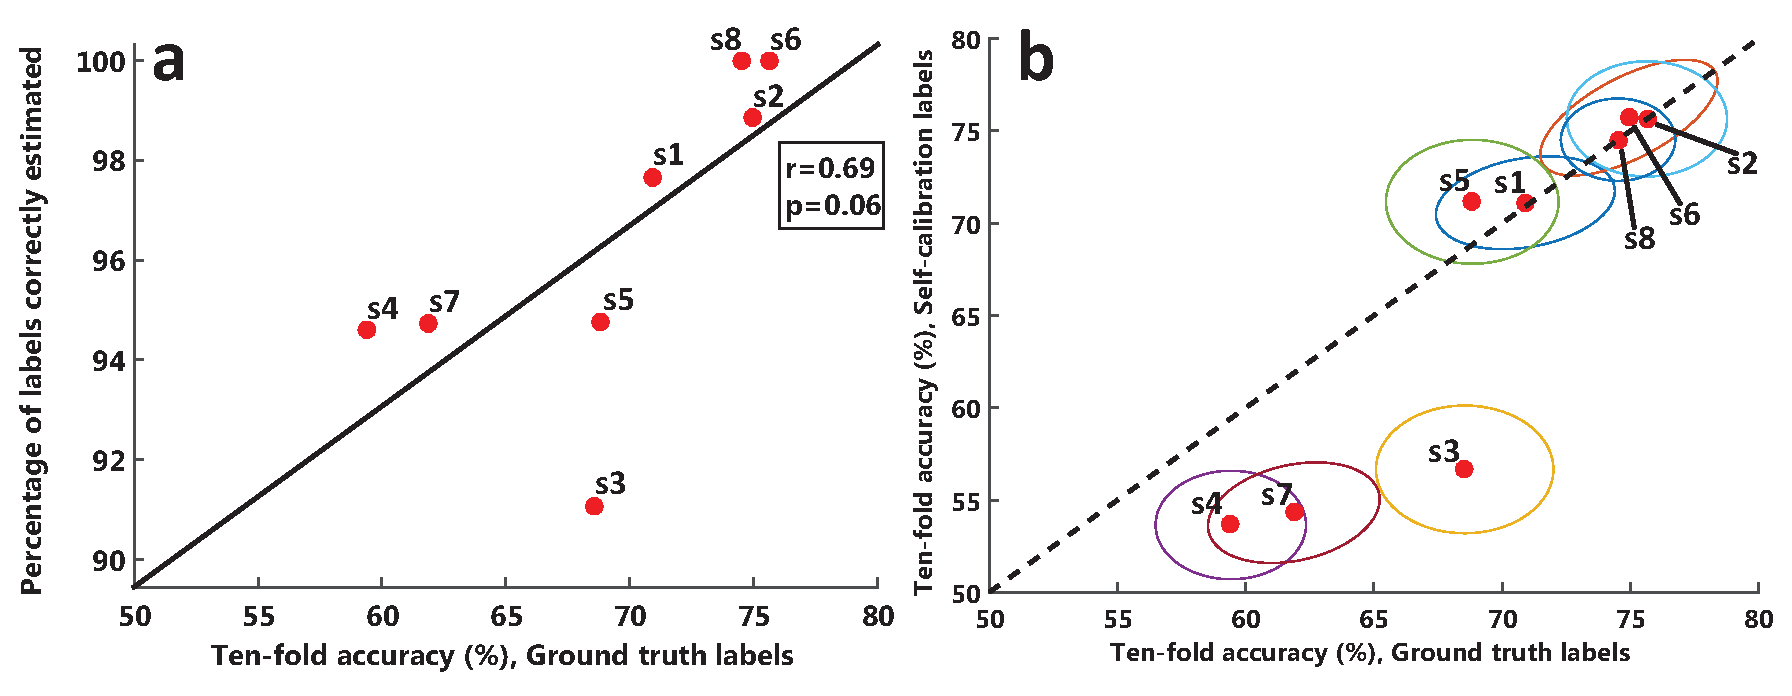
\includegraphics[width=\textwidth]{figures/figure_labels/labels_quality.eps}
\caption{\textbf{Learned labels quality}. (a) Ten-fold accuracy using the ground-truth labels (x-axis) vs percentage of the labels correctly learned by the self-calibration protocol (y-axis), together with the tendency line, where each red dot represents one subject. (b) Ten-fold accuracy using the ground-truth labels (x-axis) compared against the ten-fold accuracy using the labels learned by the self-calibration approach (y-axis). Each dot represents one subject, whereas the ellipsoid represents the uncertainty computed from the ten-fold accuracies. Every dot below (above) the dashed line implies that the self-calibration approach had worse (better) accuracies than the ground-truth labels.}
\label{fig:labels}
\end{figure*}

\subsection{Comparison with standard calibration}

Fig. \ref{fig:std_vs_sc} shows the comparison with the results obtained in our previous work (see \cite{iturrate13}) in terms of EEG signal and classification performance, based on the subjects that followed both calibration approaches (standard calibration and self-calibration). Regarding the grand-averaged signals (Fig. \ref{fig:std_vs_sc}a), no substantial differences were found on the difference potential, with only slight variations in the amplitude of the peaks. Despite small variations of around 20 ms were found in the peak latencies, these values are below our current event synchronization resolution of $62.50$ ms, and thus were mainly due to noise.

Similarly, the accuracies obtained during the online task (Fig. \ref{fig:std_vs_sc}b) following the two calibrations was significantly similar (Bonferroni-corrected unpaired t-test, $p>0.1$), demonstrating that the self-calibration approach did not result in a decrease in the classification performance. Furthermore, the performance of the self-calibration was slightly higher than that of the standard calibration, probably due to a learning effect on the user side. Fig.  \ref{fig:std_vs_sc}b also shows the number of calibration trials needed for each subject, an average of 417 trials. In the same number of trials, the zero-calibration approach allow to reach an average of 8$\pm$1 targets, and thus perform the reaching task much more efficiently.

\begin{figure*}[htbp]
\centering
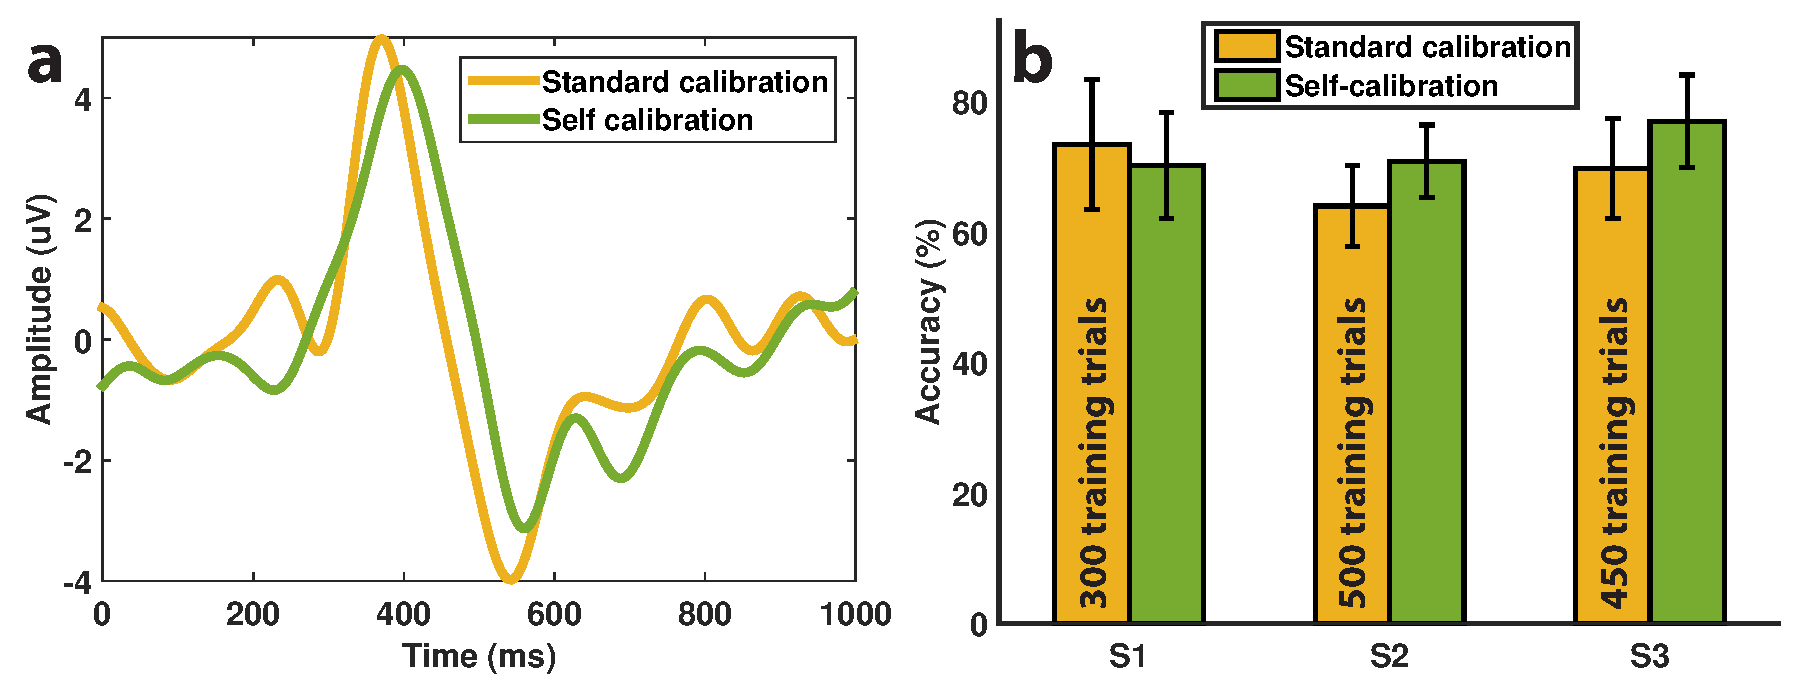
\includegraphics[width=\textwidth]{figures/standard_vs_selfcalibration.eps}
\caption{\textbf{Signal and accuracy comparison with standard calibration.} (a) Difference average (error minus correct grand averages) at channel FCz for the 3 subjects that performed the standard calibration and self-calibration protocols. (b) Online mean classification accuracy ($\pm$ std) of the three subjects after following each calibration procedure, together with the number of calibration trials used for training in the standard calibration approach.}
\label{fig:std_vs_sc}
\end{figure*}

Regarding the simulation results, Fig. \ref{fig:classification} shows the simulated training accuracies for each subject. As can be seen, the accuracies varied substantially from subject to subject, with a mean performance of $68.40\% \pm 6.69$. Nonetheless, the accuracy reached a plateau for all of them, where the mean number of calibration trials to reach this point was of $202 \pm 75$. This analysis served to run the simulations of an ErrP-based control using a supervised calibration (see Table \ref{tab:onlineXPsummary}, right). In this case, the number of correctly reached targets was significantly worse than the self-calibration approach (paired t-test, $t_{7} = -3.67, p=0.008$). The number of steps to reach the first target was also significantly worse than the steps following self-calibration ($t_{7} = -6.08, p=0.001$). Notice that for the standard calibration the number of steps to reach the first target include those steps used for supervised calibration. We can further compare the number of steps during self-calibration with the number of calibration trials. In principle, it would seem reasonable that, for those subjects needing more calibration trials, the self-calibration approach might need more trials to reach the first target. However, this hypothesis was falsified and no correlation was found ($r=0.02, p=0.97$).

\begin{figure*}[htbp]
\centering
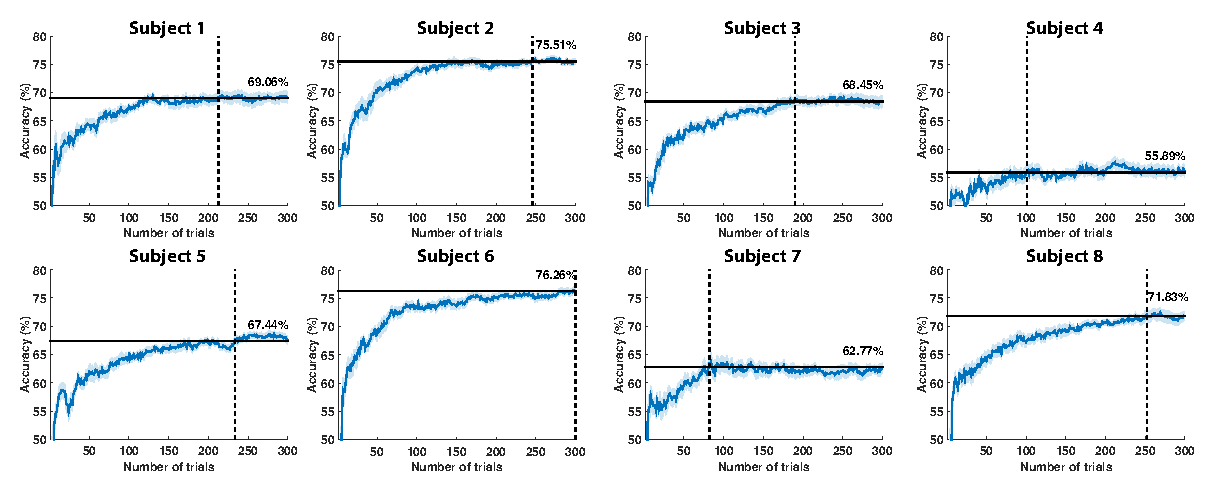
\includegraphics[width=\textwidth]{figures/classification.eps}
\caption{\textbf{Accuracy from simulated standard calibration}. Simulated calibration represented as accuracies computed by increasing the number of trials of the training dataset (x-axis) and testing the classifier with a fixed test set of 200 trials. In order to have a confidence measure (shadowed areas), this procedure was repeated 10 times while shuffling the data. The horizontal solid line represents the accuracy plateau (also shown above the line), whereas the dashed vertical line shows the number of trials needed to reach the plateau.}
\label{fig:classification}
\end{figure*}


%
%\begin{table*}
	%\centering
	%\caption{\label{tab:onlineXPsummary} Task results}
	%\rowcolors{2}{gray!25}{white}
	%\resizebox{\textwidth}{!}{
	%\begin{tabular}{ccccc|cccc|cccc}
		%\toprule
		%& \multicolumn{4}{c}{\textbf{Online self-calibration}}
		%& \multicolumn{4}{|c|}{\textbf{Simulated calibration: Fixed}}
		%& \multicolumn{4}{c}{\textbf{Simulated calibration: Subject specific}} \\ \midrule
		%\textbf{Subject} & Calib. trials & Steps $1^{st}$ & $\#$Correct & $\#$Incorrect
		%& Calib. trials & Steps $1^{st}$ & $\#$Correct & $\#$Incorrect
		%& Calib. trials & Steps $1^{st}$ & $\#$Correct & $\#$Incorrect \\ \midrule
		%\textbf{S1} & 0 & 101 & 16 & 2 & 300 & 324 & 8 & 0 & 213 & 240 & 10 & 0 \\
		%\textbf{S2} & 0 & 131 & 9 & 1 & 300 & 340 & 5 & 0 & 246 & 287 & 6 & 0 \\
		%\textbf{S3} & 0 & 265 & 3 & 1 & 300 & 411 & 1 & 0 & 190 & 324 & 2 & 0 \\
		%\textbf{S4} & 0 & 232 & 2 & 2 & 300 & 465 & 0 & 0 & 101 & 337 & 1 & 0 \\
		%\textbf{S5} & 0 & 132 & 5 & 3 & 300 & 382 & 2 & 0 & 234 & 318 & 3 & 0 \\
		%\textbf{S6} & 0 & 142 & 10 & 0 & 300 & 339 & 5 & 0 & 300 & 340 & 5 & 0 \\
		%\textbf{S7} & 0 & 79 & 4 & 3 & 300 & 451 & 0 & 0 & 82 & 310 & 0 & 0 \\
		%\textbf{S8} & 0 & 240 & 6 & 0 & 300 & 337 & 5 & 0 & 252 & 290 & 6 & 0 \\
		%\textbf{mean} & \textbf{0.00} & \textbf{165.25} & \textbf{6.88} & \textbf{1.50}
					  %& \textbf{300.00} & \textbf{381.13} & \textbf{3.25} & \textbf{0.00}
					  %& \textbf{202.25} & \textbf{305.75} & \textbf{4.13} & \textbf{0.00} \\ \bottomrule
	%\end{tabular}}
%\end{table*}
